\section

%%%%%%%%%%%%%%%%%%%%%%%%%%%%%%%%%%%%%%%%%%%%%%%%%%%%%%%%%%%%%%%%%%%%%%%%%%%%%%%
\section{Working with nonlinear petrophysical relationships} \label{LinearWithMappingSection}

\begin{figure}
    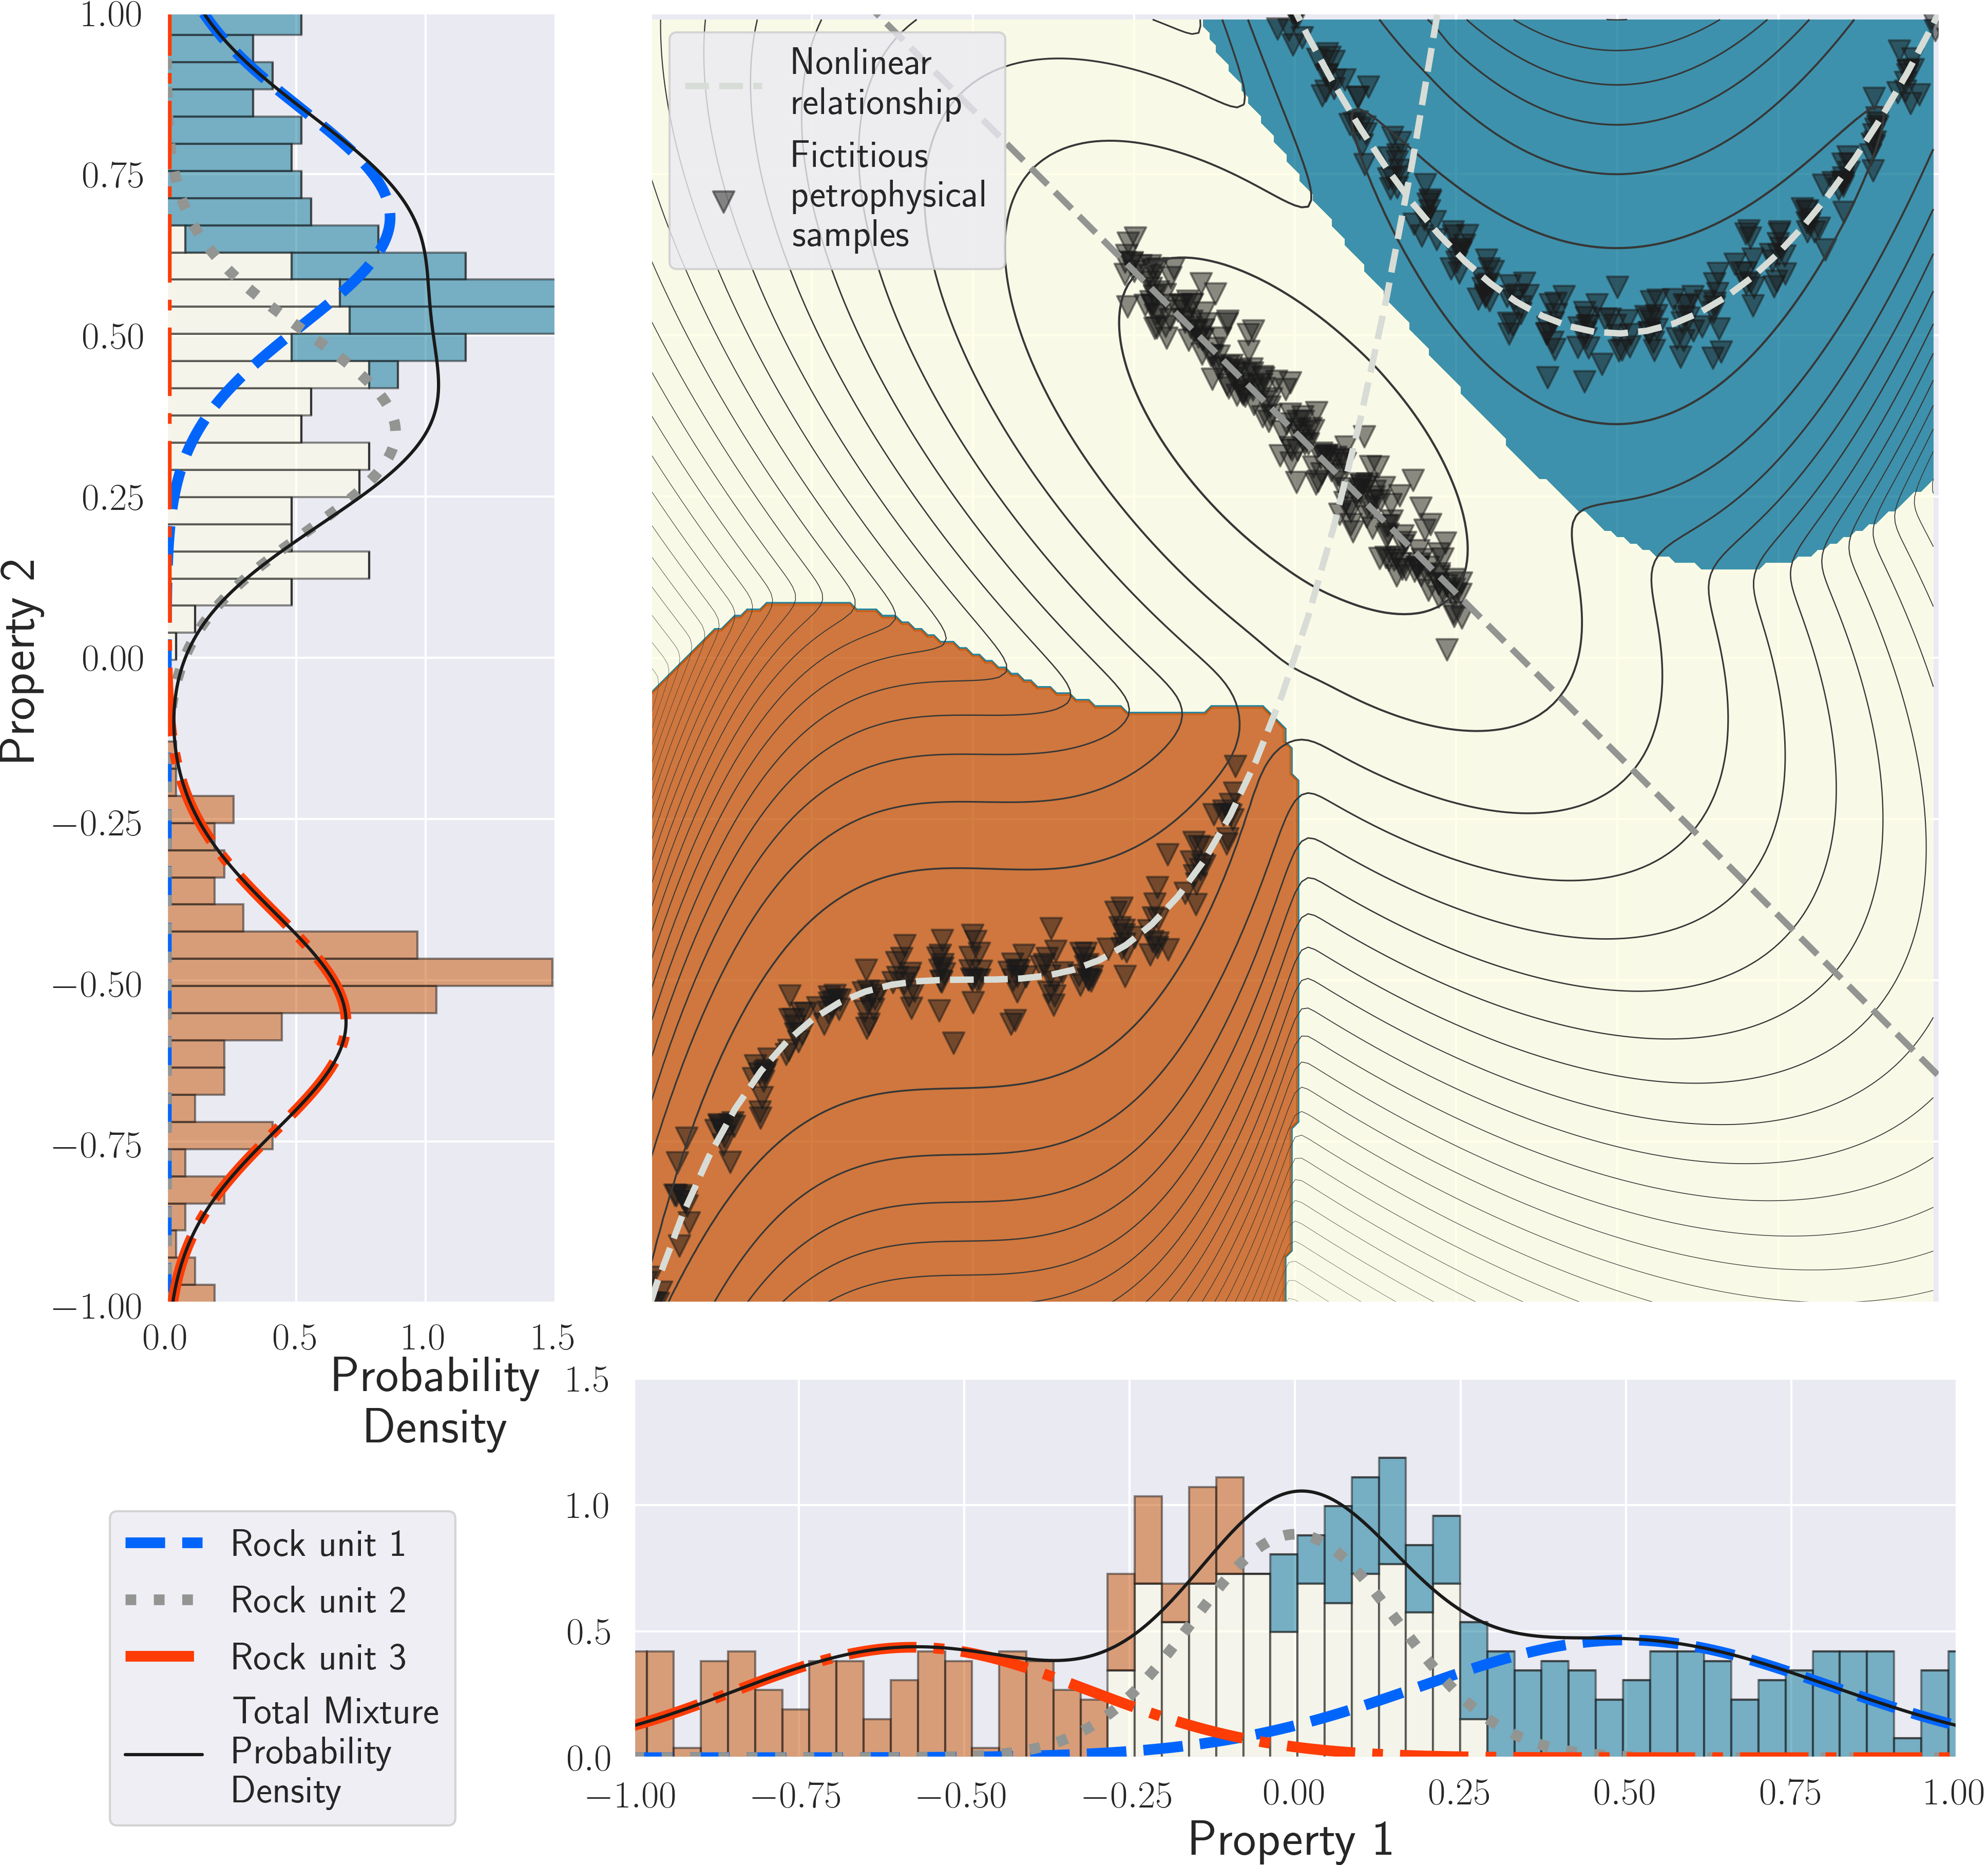
\includegraphics[width=\columnwidth]{Fig/LowRes/example_projection.png}
    \caption{GMM with various polynomial relationships: one linear (no addition required), one quadratic and one cubic. In the main panel, thicker contour lines indicate higher probabilities. The 1D probability distribution for each physical property, and the respective histogram of each unit, are projected on the left and bottom panels.}
    \label{fig:example_projection.png}
\end{figure}

While linear trends can be accounted through the covariance matrix to obtain elongated clusters, it is also possible to account for nonlinear relationships between physical properties in our framework (Fig. \ref{fig:example_projection.png}). This is achieved by composing the Gaussian function with the nonlinear relationship $P_j$ between the physical properties of the particular rock unit $j$. This corresponds to using $\mathcal{N}(P_j(\mathbf{m}_i)|\mathbf{\mu}_j, \mathbf{W}_i^{-1}\mathbf{\Sigma}_j\mathbf{W}_i^{-1})$ for each rock unit $j$ in the GMM in equation \eqref{eq:mixturemodel}.

In this section, we present a joint inversion of two linear problems whose respective physical properties have nonlinear petrophysical relationships between each other. For simplicity, the physics of the two problems is the same and is based on the example previously used in \citet{Li1996}. The models are discretized on a 1D mesh defined on the interval $[0, 1]$ and divided into 100 cells. Both datasets consist of $30$ data points at various frequencies equally distributed from $1$ to $59$ evaluated according to:
\begin{equation}
d_j = \int_0^1 e^{-jx}\cos(2\pi j x) m(x) dx, ~j=1, 3, .., 59.
\end{equation}

Each model presents three distinct units. The background for both models is set to $0$ while the two other units are linked through a quadratic and a cubic relationship respectively.

We invert the two datasets using the multi-physics PGI framework, including \textit{a priori} knowledge of the petrophysical distributions and relationships. The result can be seen in the first row of Figs \ref{fig:LinearWithMapping.png}(a) to (c). Note that the petrophysical relationships are well reproduced. This allows the recovery of details of the two models.

For comparison, we also jointly invert the datasets but without the polynomial relationships (by merely fitting a Gaussian distribution to each unit). The result can be seen in the second row of Figs \ref{fig:LinearWithMapping.png}(d) to (f). While the overall structures are well recovered, we miss some details of the models. The background is not as flat as with the full information, the lower tip of the model of problem $2$ is completely missed.

We also invert both datasets individually using the classic Tikhonov inversion. The result is shown in the last row of Figs \ref{fig:LinearWithMapping.png}(g) to (i). Results are smoother, as expected. The background presents even more variations, but the overall structures are recovered. Same as for the joint inversion without the polynomial relationships, the details are missing.

\begin{figure*}
    \includegraphics[width=\textwidth]{Fig/LowRes/LinearWithMapping.png}
    \caption{Linear joint inversions with various types of physical properties relationships (no trend, quadratic, cubic). Panels (a) to (c) show the inversion result with PGI using the known nonlinear relationships. The first panel (a) shows the result for the first problem, (b) for the second problem. The panel (c) shows the cross-plot of the models over the contour of the GMM with nonlinear relationships. Panels (d) to (f) show the result with PGI without nonlinear relationships. In panel (f), we show the used GMM without nonlinear relationships. Panels (g) to (i) show the Tikhonov inversions result.}
    \label{fig:LinearWithMapping.png}
\end{figure*}

%%%%%%%%%%%%%%%%%%%%%%%%%%%%%%%%%%%%%%%%%%%%%%%%%%%%%%%%%%%%%%%%%%%%%%%%%%%%%%%
\section{Updating the Gaussian mixture model in multi-dimensions} \label{UpdateTheta}

In this section, we generalize the learning of the GMM parameters presented in \citet{ggz389} to multivariate Gaussian distributions, representing multiple physical properties. The main difference comes from the fact that the means are now vectors (they are scalars in 1-D) and that the scalar variances in 1D become covariance matrices. We define the problem as a Maximum A Posteriori (MAP) estimate of the GMM means, proportions and covariance matrices, using the MAP Expectation-Maximization (MAP-EM) algorithm \citep{ExpectationMaximization}.
\begin{equation}
\mathcal{P}(\Theta|\mathbf{m}) \propto \mathcal{M}(\mathbf{m}|\Theta)\mathcal{P}(\Theta).
\label{theta_posterior}
\end{equation}

We choose to follow a semi-conjugate prior approach for the choice of the prior distributions $\mathcal{P}(\Theta)$ \citep{ggz389, Murphy2012}.

The computation of the responsibilities for the E-step of the MAP-EM algorithm stay the same as in \citet{ggz389}, except for the dimension of the parameters:

\begin{equation}
n_{ij}^{(k)} = \frac{\mathcal{P}(z_i=j)^{(k-1)}\mathcal{N}(\mathbf{m}_i|{\mathbf{\mu}_j}^{(k-1)}, {\mathbf{\Sigma}_j}^{(k-1)})}{ \sum_{t=1}^c \mathcal{P}(z_i=t)^{(k-1)} \mathcal{N}({\mathbf{m}}_i|{\mathbf{\mu}_t}^{(k-1)}, {\mathbf{\Sigma}_j}^{(k-1)})} \label{eq:responsibilities}.
\end{equation}
%The conjugate prior for the proportions follow a Dirichlet distribution:

The update to the proportions stays similar to the univariate case \citep{ggz389}:
\begin{align}
%&\mathcal{P}(\mathbf{\pi}) = \text{Dir}({\zeta}{\pi}_{\text{prior}}V-1) \label{pi_prior}\\
%&\text{Thus giving the update:} \nonumber \\
&{\pi}^{(k)}_j = \frac{V_{j}^{(k)}+\zeta_j {{\pi}_j}_{\text{prior}}V}{V(1+\sum_{t=1}^c \zeta_t {{\pi}_t}_{\text{prior}})} \label{eq:pi_update}, \\
&\text{with:} \nonumber\\
&V_{j}^{(k)} = \sum^n_{i=1} v_i n_{ij}^{(k)}, \label{VolumeProportions}\\
&\text{ and } V=\sum^n_{i=1} v_i,
\end{align}
where $\zeta_j$ is the confidence in the prior proportion ${\pi_j}_{\text{prior}}$ of the rock unit $j$, $v_i$ is the volume of the $i$\textsuperscript{th} cell and $V$ is the volume of the
active mesh. This allows the estimates to be mesh-independent by using volumetric proportions instead of cell counts.

%The semi-conjugate for the means and covariance matrices follow respectively a Gaussian and Inverse-Wishart distributions:
%\begin{align}
%&\mathcal{P}(\mathbf{\mu}| \mathbf{\Sigma}) = \mathcal{N}(\mathbf{\mu}|\mathbf{\mu}_{\text{prior}}, \text{diag}(\mathbf{\kappa}\pi_{\text{prior}}V)^{-1} \Sigma) \label{mu_semiprior} \\
%&\text{and:}\nonumber \\
%&\mathcal{P}(\mathbf{\Sigma}|\mathbf{\mu}) = \mathcal{W}^{-1}(\mathbf{\Sigma}|({\nu}{\pi}_{\text{prior}}V)\mathbf{\Sigma}_{\text{prior}}, {\nu}{\pi}_{\text{prior}}V-q-1) \label{sigma_semiprior}
%\end{align}

The mean update proposed in \citet{ggz389} generalizes to each physical property $p$:
\begin{align}
&{\mu_j^p}^{(k)}=\frac{V_{j}^{(k)}{\bar{{m}^p_j}}^{(k)} + \kappa^p_j {\pi_j}_{\text{prior}} V {\mu^p_j}_{\text{prior}}}{V_{j}^{(k)}+\kappa_j^p {\pi_j}_{\text{prior}} V} \label{eq:mu_update},\\
&\text{with:} \nonumber\\
&{\bar{\mathbf{m}}}_j^{(k)} = \frac{\sum^n_{i=1} v_i n_{ij}^{(k)} \mathbf{m}_i}{V_{j}^{(k)}},
\end{align}
where $\kappa_j^p$ is the confidence in ${{\mu^p_j}_{\text{prior}}}$, which is the prior mean of the physical property $p$ of the rock unit $j$. The confidences $\{\mathbf{\kappa}\}$ are thus consider as vectors. This is an important tool that we use in section \ref{sec:InterpreterAssumption} to formulate a geologic assumption about the model.

The update to the covariance matrices is, with $\nu_j$ the confidence in the prior covariance matrix ${\mathbf{\Sigma}_j}_{\text{prior}}$ of the rock unit $j$:
\begin{align}
&{\mathbf{\Sigma}_j}^{(k)} = \frac{{{V_{j}^{(k)}} {\mathbf{\Sigma}_{\bar{\mathbf{m}}}}_j}^{(k)} + \nu_j {\pi_j}_{prior} V {\mathbf{\Sigma}_j}_{prior}}
{{V_{j}^{(k)}} + \nu_j {\pi_j}_{prior} V} \label{eq:sig_update},\\
&\text{with:} \nonumber\\
&{\mathbf{\Sigma}_{\bar{\mathbf{m}}}}_j^{(k)} =\frac{1}{{V_{j}^{(k)}}} \sum_{i=1}^{n} v_i n_{ij}^{(k)}(\mathbf{m}_i-\bar{\mathbf{m}_j}^{(k)})(\mathbf{m}_i-\bar{\mathbf{m}_j}^{(k)})^\top,
\end{align}

%%%%%%%%%%%%%%%%%%%%%%%%%%%%%%%%%%%%%%%%%%%%%%%%%%%%%%%%%%%%%%%%%%%%%%%%%%%%%%%
\section{Algorithm} \label{algorithm}

\begin{algorithm*}
    \small
    \SetKwInOut{Initialization}{Initialization}
    \caption{PGI extended from \citet{ggz389} for joint inversion}
    \label{algo:algorithm}
    \nl \Initialization{
    \begin{itemize}
    \item \underline{Input:}
    \begin{itemize}
        \item Initial geophysical model $\mathbf{m}^{(0)}$, GMM parameters $\Theta^{(0)}$ and geological model $\mathbf{z}^{(0)}$.
    \end{itemize}

    \item \underline{Parameters:}
    \begin{itemize}
      \item \textit{Objective function}: data's noise $\left\{{\mathbf{W}_d}_p\right\}_{p=1..q}$, $\beta^{(0)}$ and $\left\{\alpha\right\}$.parameters.
      \item \textit{Localized prior}: specific $\mathcal{P}(z_i)$ for available locations $i \in \{1..n\}$, weights $\left\{\mathbf{w}\right\}$.
      \item \textit{GMM prior weights}: $\left\{\mathbf{\kappa}_j, \nu_j, \zeta_j\right\}_{j=1..c}$ for the means, variances and proportions.
      \item \textit{Optimization}: $\beta$-cooling factor $\gamma$ ($> 1$), sufficient decrease rate $\tau$ ($\leq 1$), tolerance on target misfit $\epsilon$.
    \end{itemize}

    \item \underline{Output:}
    \begin{itemize}
        \item $\mathbf{m}$, $\Theta$, $\mathbf{z}$.
    \end{itemize}

    \end{itemize}
    }

    \While{$\text{any}({{\Phi_d^k}}>{{\Phi_d^k}^*}, k=1..r)$ and $\Phi_{\text{petro}}>\Phi_{\text{petro}}^*$}{

        \underline{Objective Function Descent Step:}
        \begin{itemize}
        \item Compute a model perturbation $\delta \mathbf{m}$ using an inexact Gauss-Newton.
        \item Line search with Wolfe condition to find an $\eta$ that satisfy a sufficient decrease of $\Phi$.
        \item Return $\mathbf{m}^{(t)} = \mathbf{m}^{(t-1)}+\eta \delta \mathbf{m}$.
        \end{itemize}

        \nl \underline{Update Petrophysical Distribution}
        \begin{itemize}
        \item Fit a new GMM $\Theta^{(t)}$ on $\mathbf{m}^{(t)}$ such as in equations \eqref{eq:pi_update}, \eqref{eq:mu_update} and \eqref{eq:sig_update} until no sufficient increase of the posterior is observed.
        \end{itemize}

        \nl \underline{Classification:}
        \begin{itemize}
        \item Compute the membership $\mathbf{z}^{(t)}$ of the current model $\mathbf{m}^{(t)}$ as in equation \eqref{eq:membership} using $\Theta^{(t)}$.
        \item Update $\mathbf{m}_{\text{ref}}$ and $\mathbf{W}_s$ according to equations \eqref{eq:mref_update} and \eqref{eq:Ws_update} respectively using $\mathbf{z}^{(t)}$.
        \end{itemize}

        \nl \underline{Update regularization weights:}\\
        \uIf{$\text{all}({\Phi_d^k}^{(t)}\geq\text{max}((1+\epsilon){\Phi_d^k}^*, \tau {\Phi_d^k}^{(t-1)}), k=1..r)$}{
        Decrease $\beta$: $\beta^{(t)}=\frac{\beta^{(t-1)}}{\gamma}$.
        }
        \uElseIf{$\text{all}({\Phi_d^k}^{(t)}\leq{\Phi_d^k}^*, k=1..r)$ and $\Phi_{\text{petro}}>\Phi_{\text{petro}}^*$}{
              Increase $\alpha_s$: $\alpha_s^{(t)}=\alpha_s^{(t-1)} \times \text{median}(\frac{{{\Phi_d^k}^*}}{{{{{\Phi_d^k}}}^{(t)}}}, k=1..r)$ (equation \eqref{eq:alpha_warm}).
        }
        \uIf{(optional) $\text{all}({\Phi_d^k}^{(t)}\leq{\Phi_d^k}^*)$ and $\Phi_{\text{petro}}>\Phi_{\text{petro}}^*$ and $\mathbf{z}^{(t)}==\mathbf{z}^{(t-1)}$}{
        Include $\mathbf{m}_{\text{ref}}$ in Smoothness.
        }

        \nl \underline{Update geophysical data misfit weights:}\\
        \uIf{$\text{any}({\Phi_d^k}^{(t)}\leq {\Phi_d^k}^*, k=1..r)$}{
          update $\left\{\chi\right\}$ according to equations \eqref{eq:chi_update} to \eqref{eq:chi_normalizing}.
        }

    }
\end{algorithm*}


%%%%%%%%%%%%%%%%%%%%%%%%%%%%%%%%%%%%%%%%%%%%%%%%%%%%%%%%%%%%%%%%%%%%%%%%%%%%%%%
\section{Pseudo-code for the implementation in SimPEG} \label{pseudocode}

Here, we provide an overview for the use of our implementation of the multi-physics PGI framework by other scientists. We outline the main components of the multi-physics PGI implementation using \texttt{SimPEG} and other core tools in the Python ecosystem. As in the paper, we consider the multi-physics inversion of gravity and magnetic data.

We begin by creating a simulation \texttt{mesh} and defining mappings that translate the model vector, which contains all of the parameters we will invert for, to physical properties on the mesh to be used in each forward simulation. The inversion model is a single vector; for an inversion with multiple physical parameters, we stack them and use the \texttt{Wires} map to keep track of which indices in the vector correspond to each physical parameter.
\usestyle{default}
\includecode{model_mappings.py}
%{\small\begin{verbatim}
%import numpy as np
%import discretize  # construct a simulation mesh with discretize
%from SimPEG import maps

%# model vector with size 2 * number of cells
%initial_model = np.hstack([model_grav, model_mag])

%# the Wires map selects the indices in the vector that correspond to.
%wires = maps.Wires(("density", mesh.nC), ("susceptibility", mesh.nC))
%\end{verbatim}
%}

Note that mappings can be composed; for example if we wanted to invert for log-susceptibility rather than susceptibility, then we would compose the \texttt{wires.susceptibility} mapping with an \texttt{ExpMap} instance. For examples, see \citet{SeogiMapping}.


Next, we construct the forward simulations for both the gravity and magnetic data. The \texttt{survey} objects contain the locations of the receivers as well as parameters defining the source field for the magnetics simulation (magnitude, inclination, and declination).
\usestyle{default}
\includecode{data_misfits.py}

% I don't think these details are crucial

% # set up the gravity surveys
% grav_receivers = gravity.receivers.Point(grav_rx_locs)
% grav_source = gravity.sources.SourceField([grav_receivers])
% grav_survey = gravity.GravitySurvey([grav_source])

% # set up the magnetic surveys
% mag_receivers = magnetics.receivers.Point(mag_rx_locs)
% mag_source = magnetics.sources.SourceField([mag_receivers])
% mag_survey = magnetics.MagneticsSurvey([mag_source])


%{\small\begin{verbatim}
%from SimPEG.potential_fields import gravity
%from SimPEG.potential_fields import magnetics

%# construct the gravity simulation
%grav_simulation = gravity.Simulation3DIntegral(
%    mesh, map_density=wires.density, survey=grav_survey
%)

%# construct the magnetics simulation
%mag_simulation = magnetics.Simulation3DIntegral(
%    mesh, map_susceptibility=wires.susceptibility, survey=mag_survey
%)
%\end{verbatim}
%}

With both gravity and magnetic simulations defined, we now have the ability to compute predicted data given a model. The next step is to construct the data misfit term as described in equation \eqref{eq:datamisfit}. 
\usestyle{default}
\includecode{combodatamisfit.py}
%{\small\begin{verbatim}
%from SimPEG import data_misfit

%# Construct the geophysical data misfits
%phi_grav = data_misfit.L2DataMisfit(simulation=grav_simulation, data=grav_data)
%phi_mag = data_misfit.L2DataMisfit(simulation=mag_simulation, data=mag_data)

%# Combine to create the whole data misfit
%phi_data = chi_grav * phi_grav + chi_mag * phi_mag
%\end{verbatim}
%}

The \texttt{mag\_data} and \texttt{grav\_data} objects contain the observed data as well as user-specified uncertainties, and the scalar \texttt{chi}-values are initialized according to equation \eqref{eq:chi_normalizing}.

Next, we construct the GMM and regularization which consists of the petrophysical smallness term described in equation \eqref{eq:smallness_petro} and smoothness terms for both the density and susceptibility. To construct the GMM, we use the \texttt{WeightedGaussianMixtureModel} object, which inherits from and extends the \texttt{sklearn.mixture.GaussianMixture} object in Scikit-Learn \citep{scikit-learn}. The instantiated \texttt{gmm} object has methods for fitting a GMM on a model and computing membership of a model as needed in steps 4 and 5 in Algorithm \ref{algo:algorithm}.
\usestyle{default}
\includecode{regularization.py}

% Thibaut - you may want to add some more verbage here



%{\small\begin{verbatim}

%from SimPEG import regularization
%from SimPEG.petrophysics import WeightedGaussianMixtureModel

%gmm = WeightedGaussianMixtureModel(
%    n_components=3,  # number of rock units
%    mesh=mesh,
%    means_init=initial_means,
%    covariances_init=initial_covariances,
%)

%pgi_smallness = regularization.Petrophysical(
%    mesh=mesh,
%    mref=initial_model,
%    gmm_prior=gmm,
%    wires_map=wires,
%    cell_weights=sensitivity_weights
%)

%# smoothness terms are constructed using regularization.SmoothDeriv class
%phi_m = (
%    alpha_s * pgi_smallness +
%    alpha_smooth_grav * smoothness_grav +
%    alpha_smooth_mag * smoothness_mag
%)

%\end{verbatim}
%}

Having defined the components of the objective function, we now specify the optimization routine, in this case, inexact Gauss Newton with projections for bound constraints.
\usestyle{default}
\includecode{optimization.py}
%{\small\begin{verbatim}
%from SimPEG import optimization, inverse_problem

%# Define the optimization routine and model bounds
%opt = optimization.ProjectedGNCG(
%    lower_bound=lower_bound, upper_bound=upper_bound
%)

%# Inverse problem
%inv_prob = inverse_problem.BaseInverseProblem(phi_d, phi_m, opt)

%\end{verbatim}
%}

Finally, we assemble the inversion using \texttt{directives} in SimPEG to orchestrate updates throughout the inversion. Each directive has an \texttt{initialize} method which is called at the beginning of the inversion and can be used to set initial values of parameters, for example to initialize $\beta$ and the $\alpha$-values, as well as an \texttt{end\_iteration} method which is called after a model update (at the end of step 3 in Algorithm \ref{algo:algorithm}) and can be used to update parameters in the inversion. The updates in steps 4 through 7 in Algorithm \ref{algo:algorithm} make use of the \texttt{directives} functionality.
\usestyle{default}
\includecode{inverse_problem.py}
%{\small\begin{verbatim}
%from SimPEG import inversion, directives

%# Inverse problem with directives
%inv = inversion.BaseInversion(
%    inv_prob,
%    directives=[
%        estimate_beta0,
%        estimate_alphas,
%        target_misfits,
%        update_classification,
%        update_regularization_weights,
%        include_mref_in_smoothness,  # optional
%        update_geophysical_misfit_weights,
%    ]
%)

%recovered_model = inv.run(initial_model)

%\end{verbatim}
%}

%%%%%%%%%%%%%%%%%%%%%%%%%%%%%%%%%%%%%%%%%%%%%%%%%%%%%%%%%%%%%%%%%%%%%%%%%%%%%%%
\section{Additional models obtained by PGIs for the DO-$27$ synthetic case study} \label{sec:additionalIndividual}

\begin{figure}
\centering
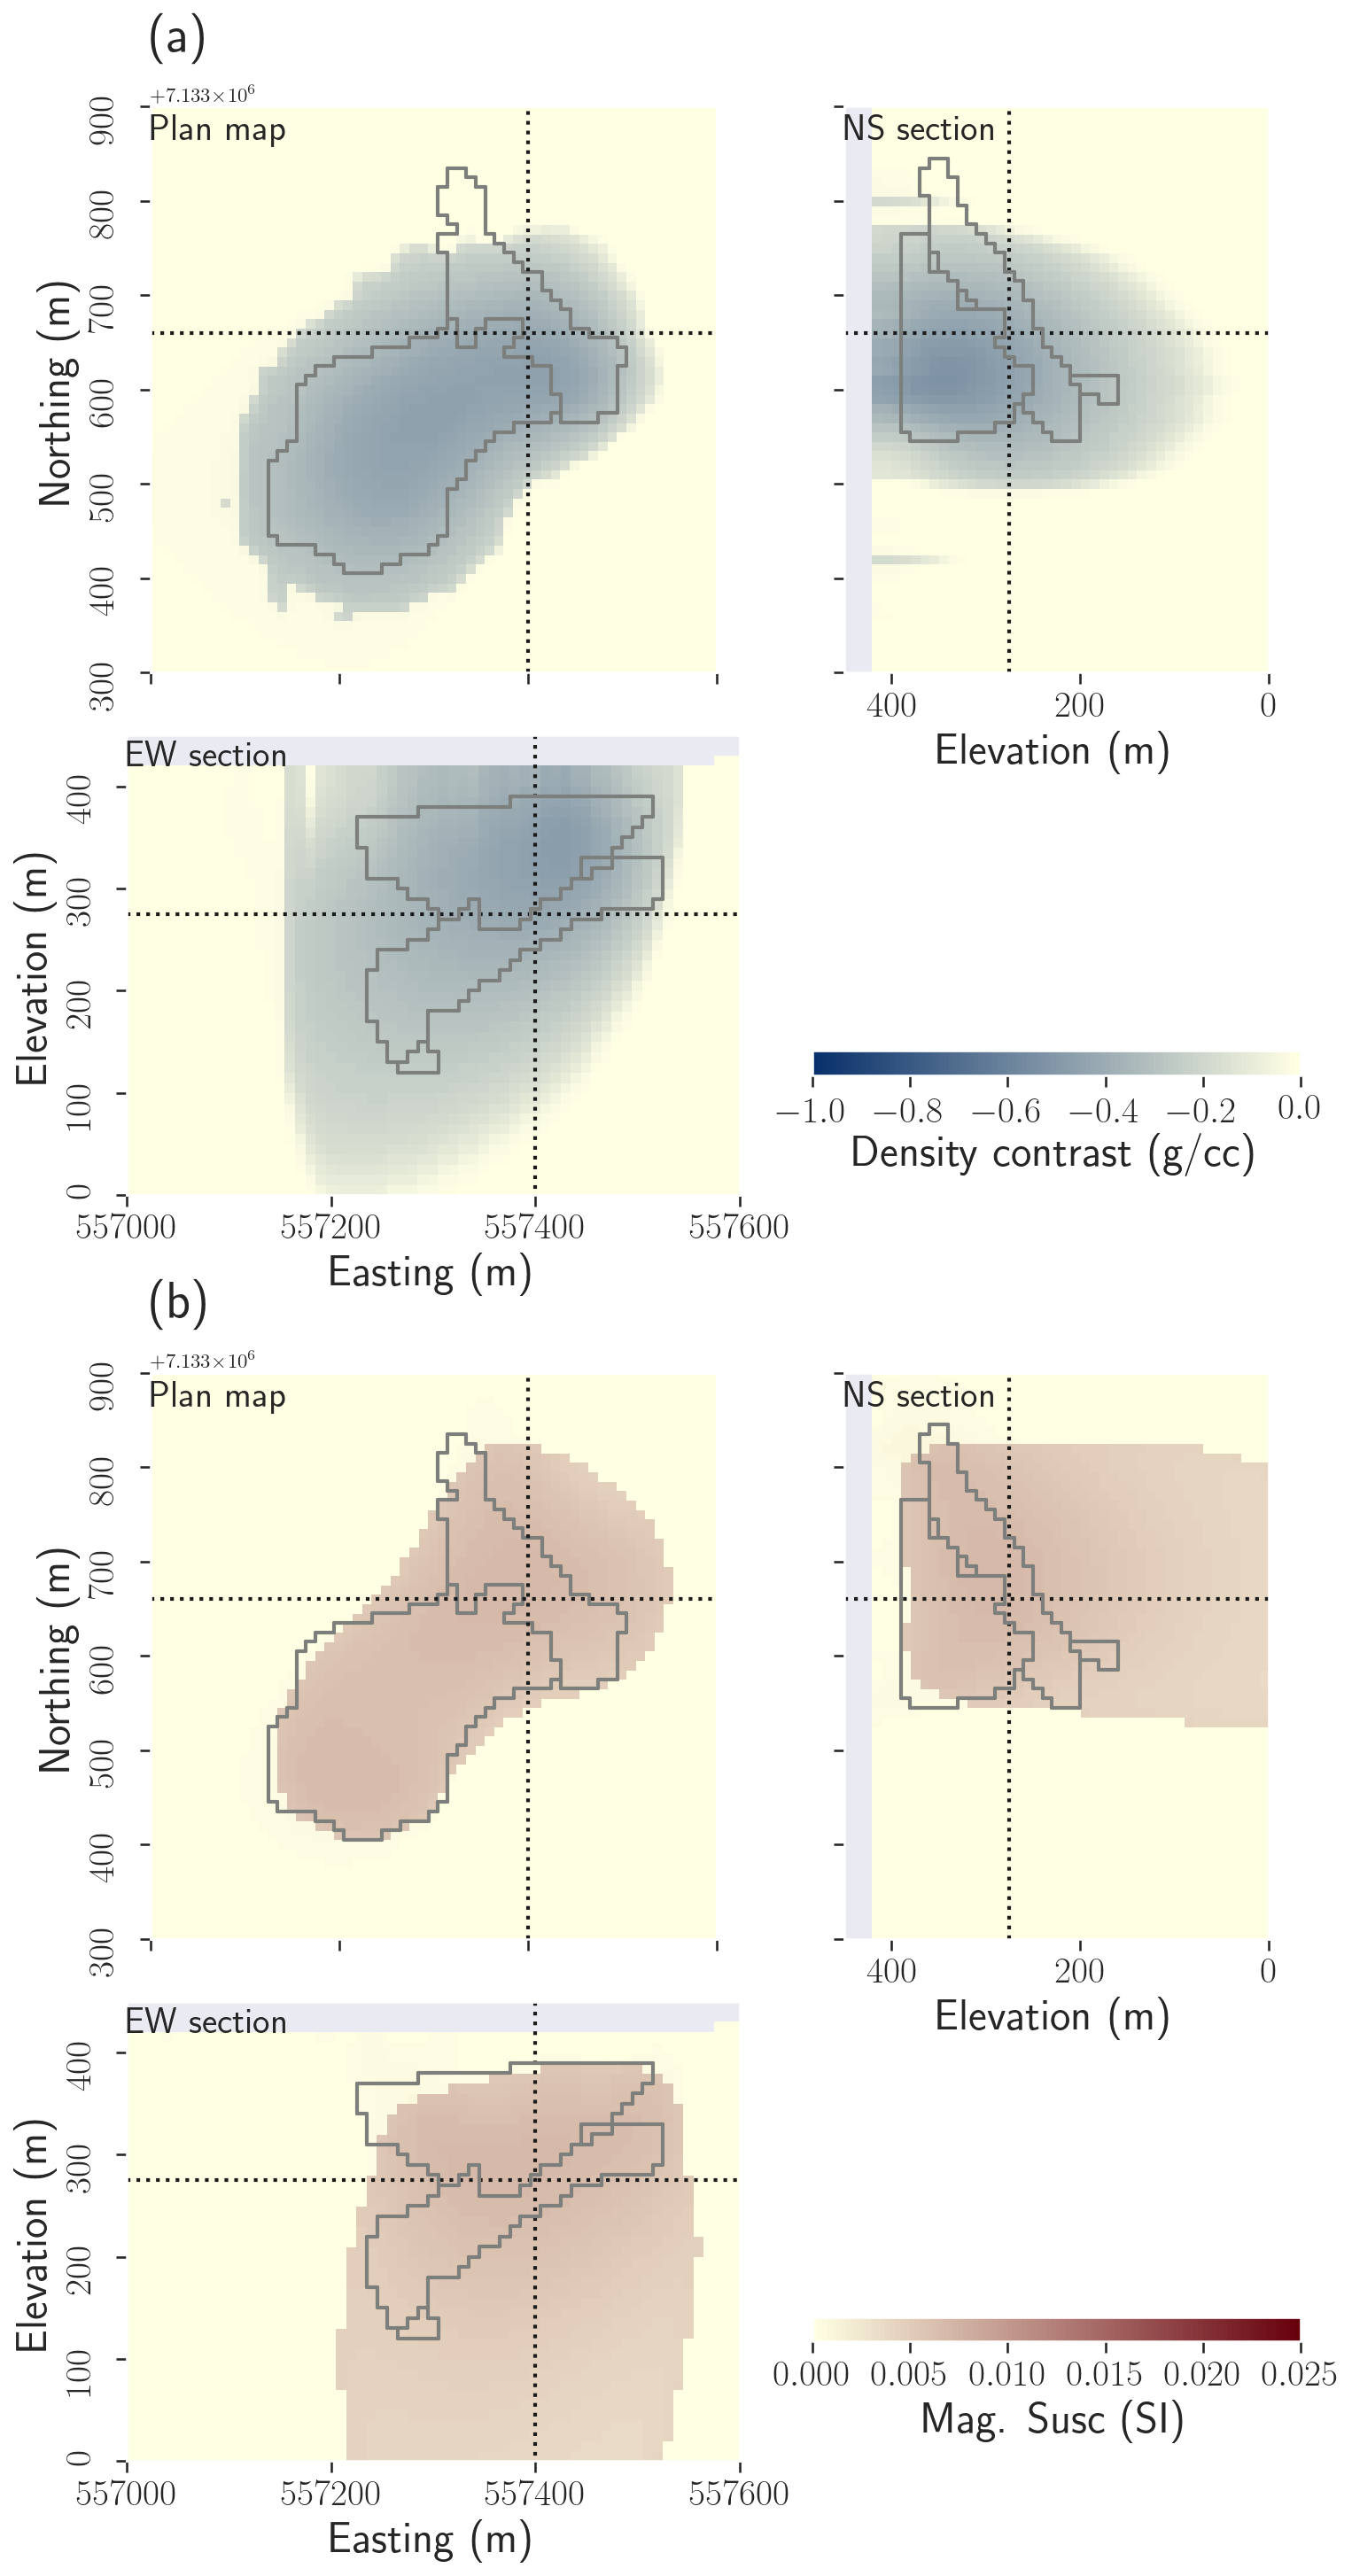
\includegraphics[width=0.5\textwidth]{TKC_AdditionalIndividualPetro_FULL_Synthetic.png}
\caption{(a) magnetic PGI using PK/VK magnetic signature. Note that the recovered volume is much larger than the volume of PK/VK recovered from the gravity inversion with this unit density contrast (Fig. \ref{fig:TKC_IndividualPetro_Synthetic.png}c); (b) gravity PGI using the HK density contrast signature. Note again the larger volume compared to Fig. \ref{fig:TKC_IndividualPetro_Synthetic.png}(d).}
\label{fig:TKC_AdditionalIndividualPetro_FULL_Synthetic.png}
\end{figure}

%%%%%%%%%%%%%%%%%%%%%%%%%%%%%%%%%%%%%%%%%%%%%%%%%%%%%%%%%%%%%%%%%%%%%%%%%%%%%%%
%\section{Multi-physics PGI with no petrophysical information and no assumption} \label{sec:twoclusters}

\begin{figure*}
    \centering
    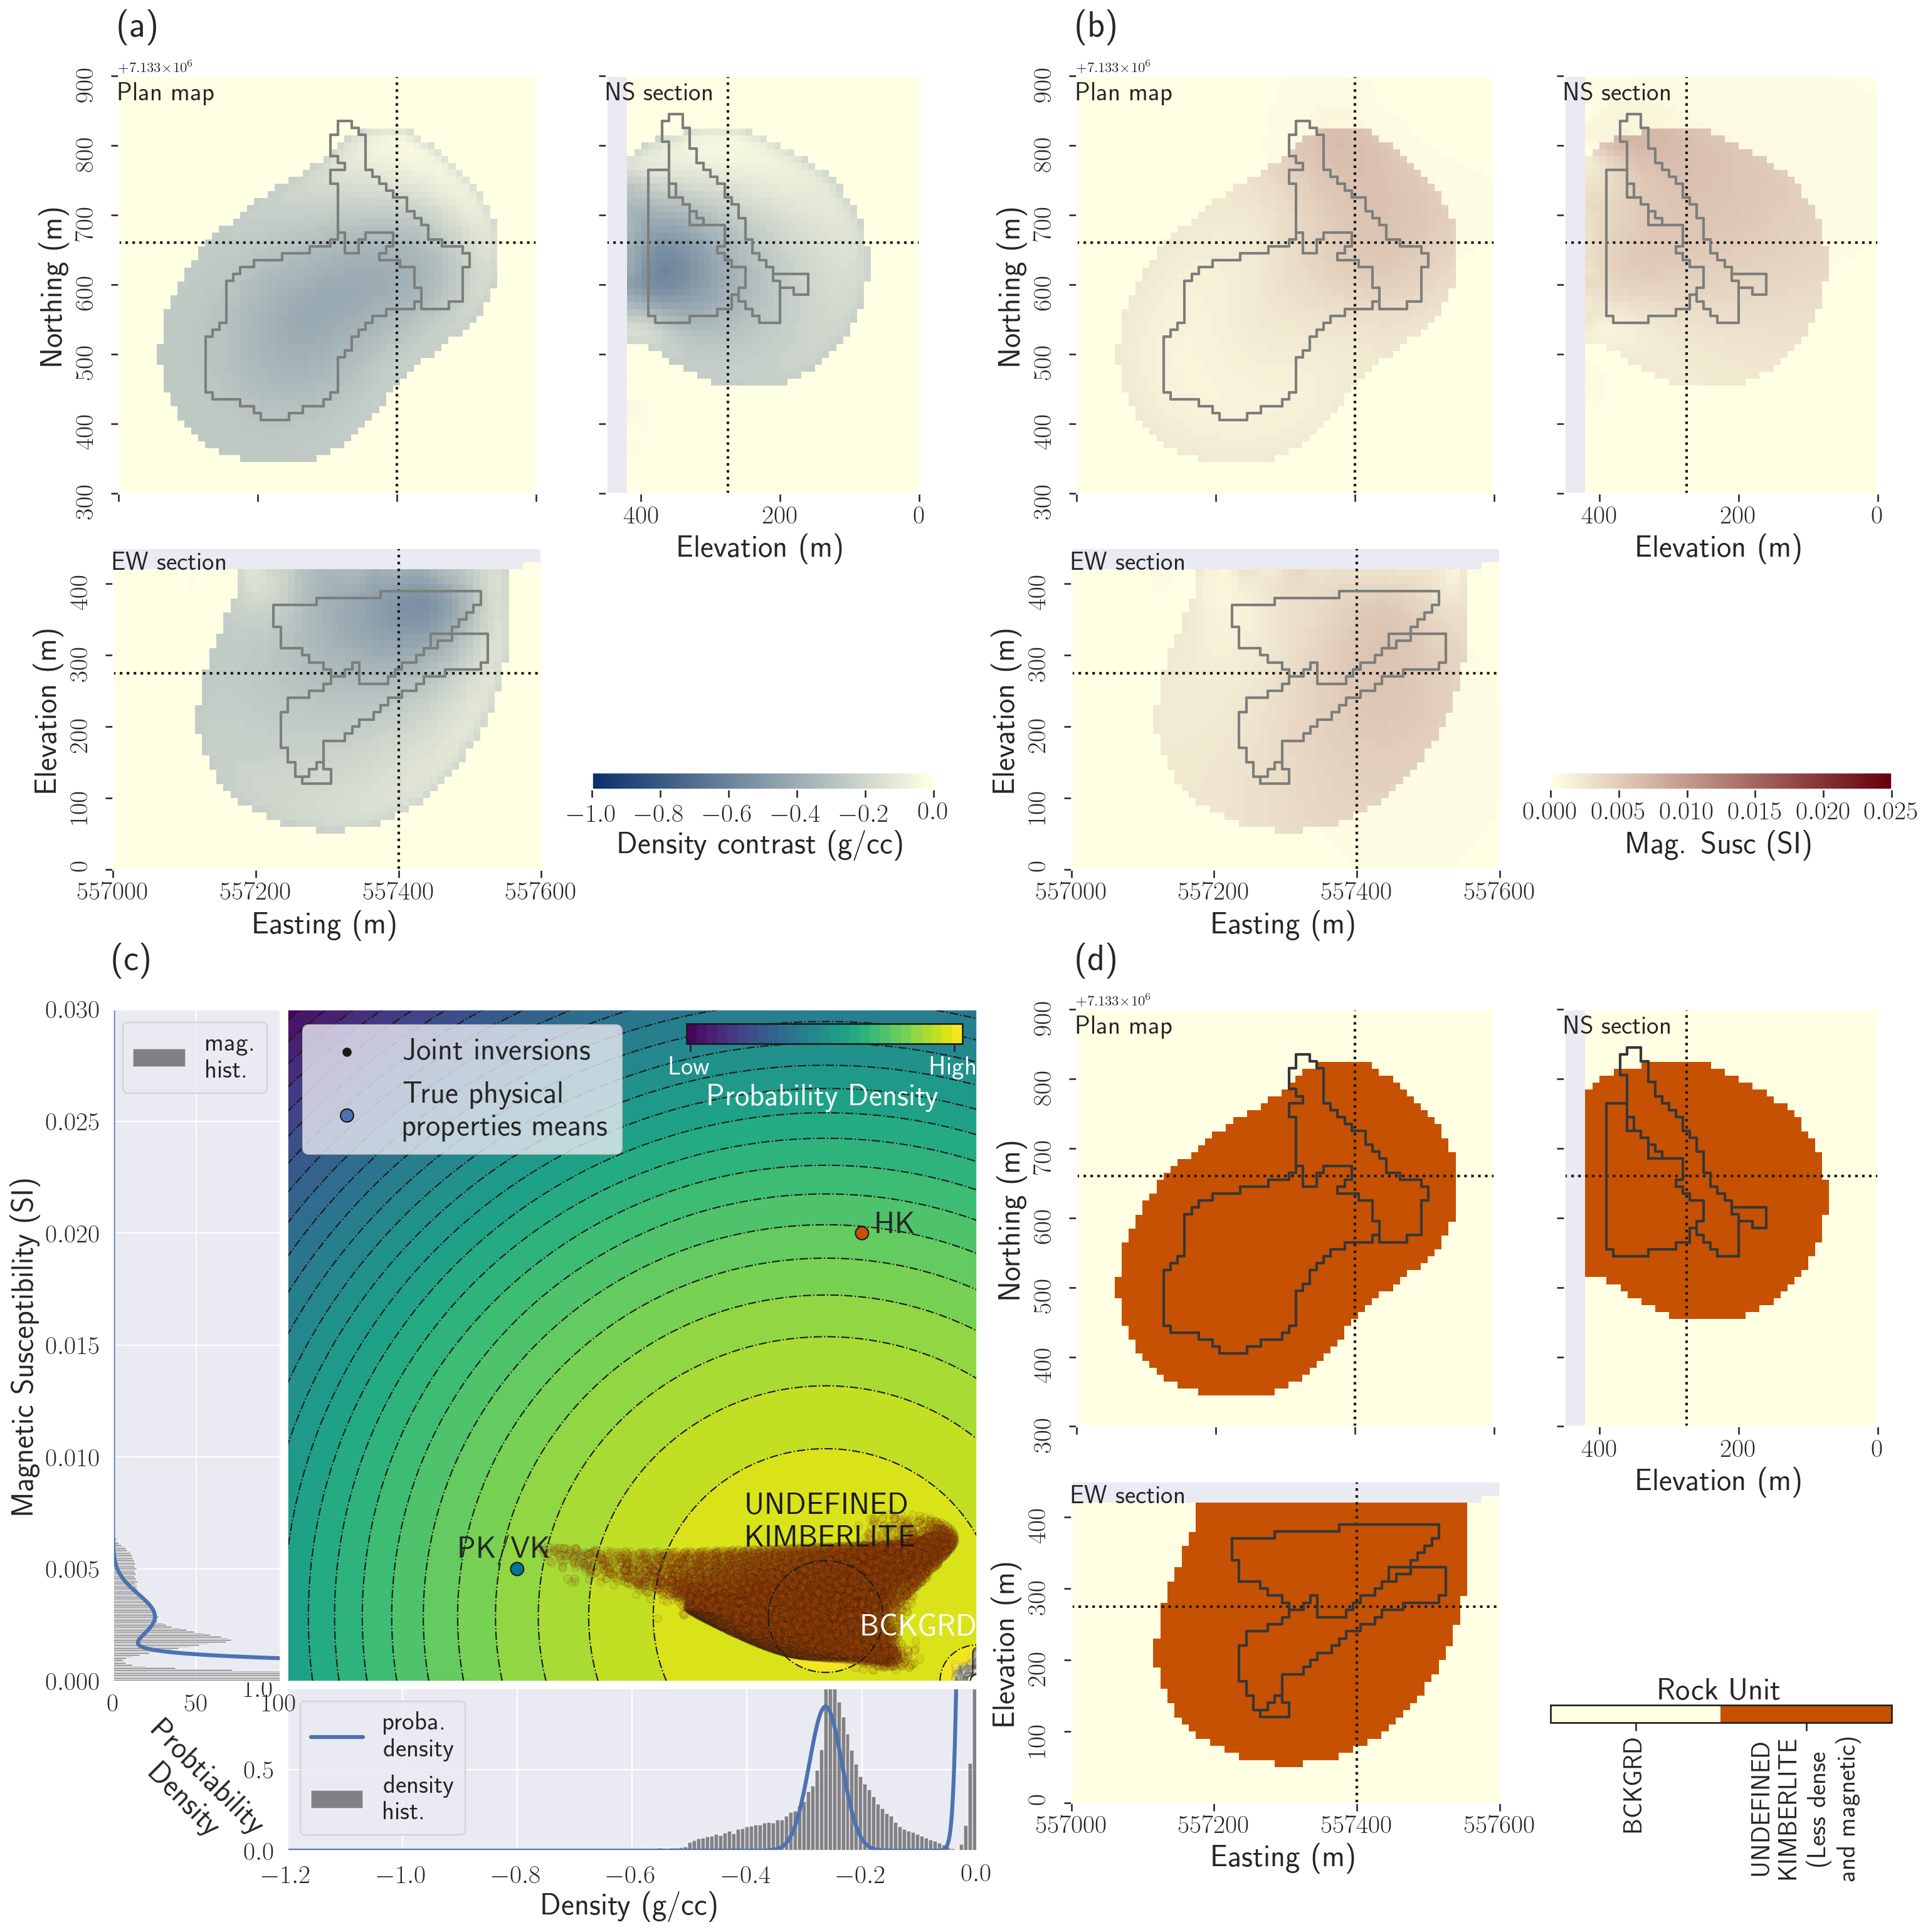
\includegraphics[width=\textwidth]{Fig/LowRes/TKC_NoPrior_Synthetic.png}
    \caption{Results of the multi-physics PGI without providing the means of the physical properties for the kimberlite facies; a single kimberlite body is enough to meet the petrophysical requirements (the spread set by the covariances matrices) and reproduce the geophysical datasets; (a) Plan map, East-West and North-South cross-sections through the recovered density contrast model; (b) Plan map, East-West and North-South cross-sections through the magnetic susceptibility contrast model; (c) Cross-plot of the inverted models. The colour has been determined by the clustering obtained from this framework joint inversion process. In the background and side panels, we show the learned petrophysical GMM distribution; (d) Plan map, East-West and North-South cross-sections through the resulting quasi-geology model.}
    \label{fig:TKC_NoPrior_Synthetic.png}
\end{figure*}
